\section{Results}

\subsubsection{Motivational R-side measurements}

\begin{figure}[!htbp]
  \centering
  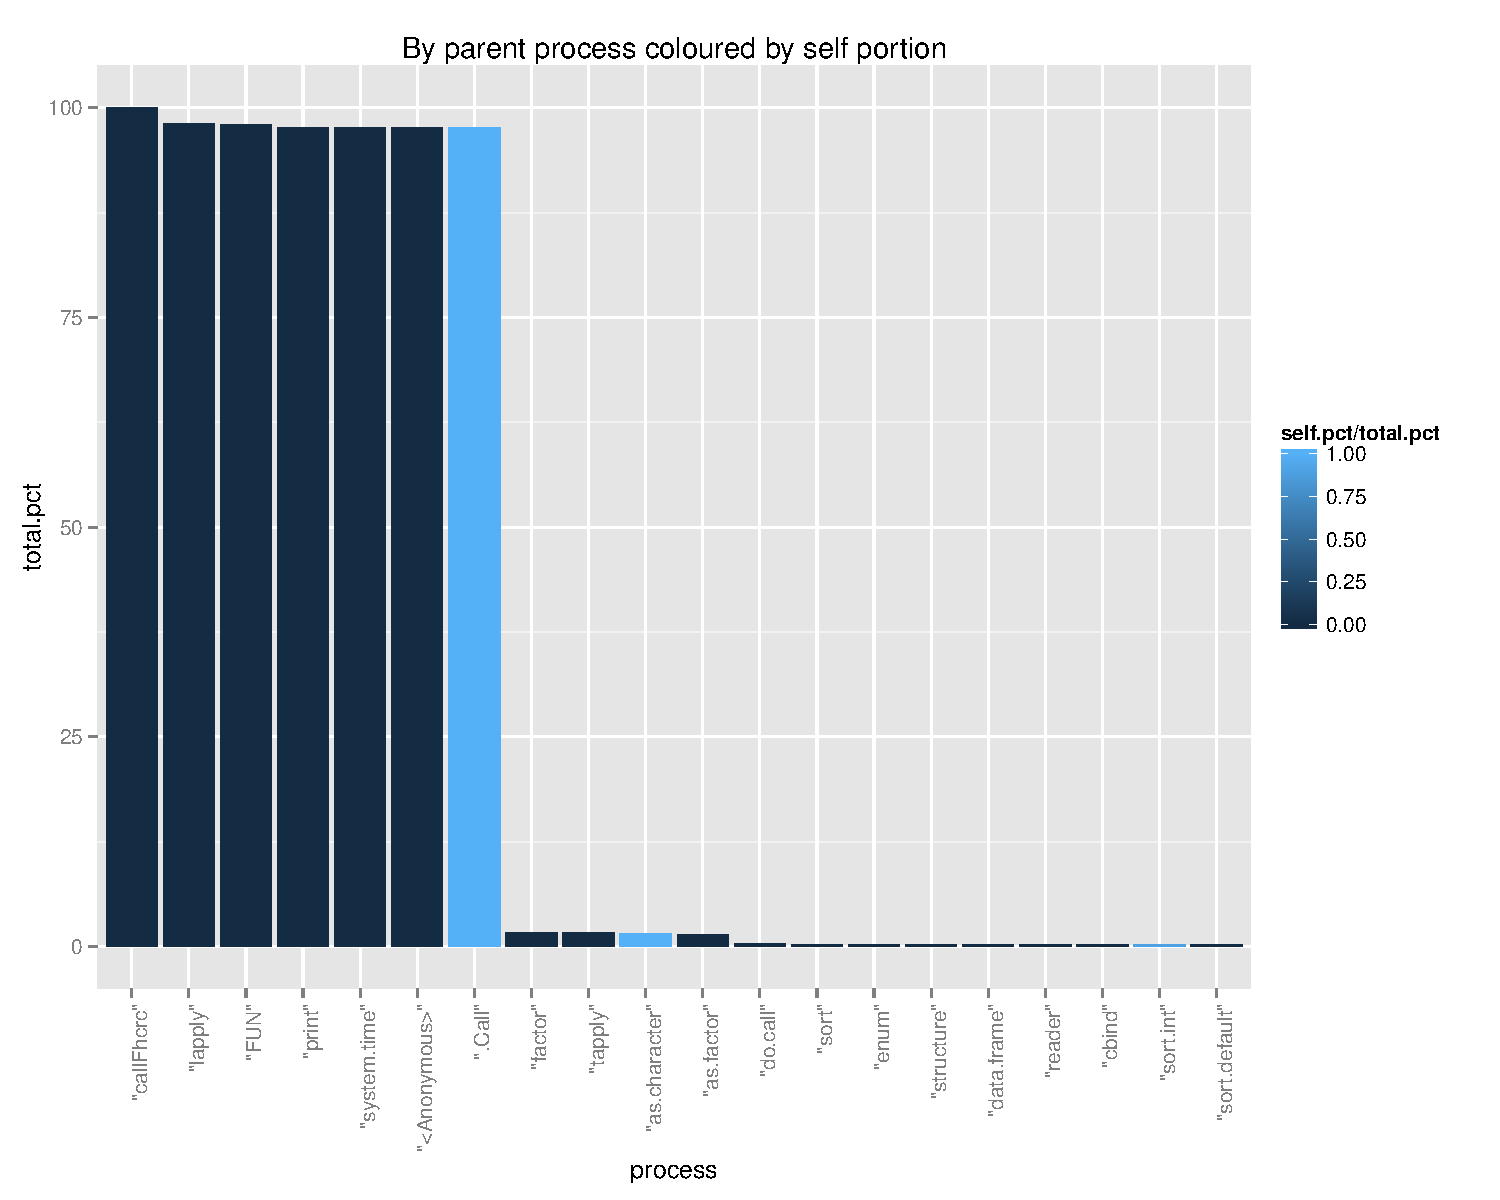
\includegraphics[width=0.7\textwidth]{images/parentColByPortion.pdf}
  \caption{Performance testing on the R side, where the ".Call" is
    the C++-code which can be run in parallel.}
  \label{fig:Rself}
\end{figure}

To motivate the need and choice to go parallel Figure \ref{fig:Rself})
shows the processes from the R-side where ".Call" is the part
which is implemented in C++ and which can be run in parallel.

\subsection{Baseline measurements C++}

\begin{figure}[!htbp]
  \centering
  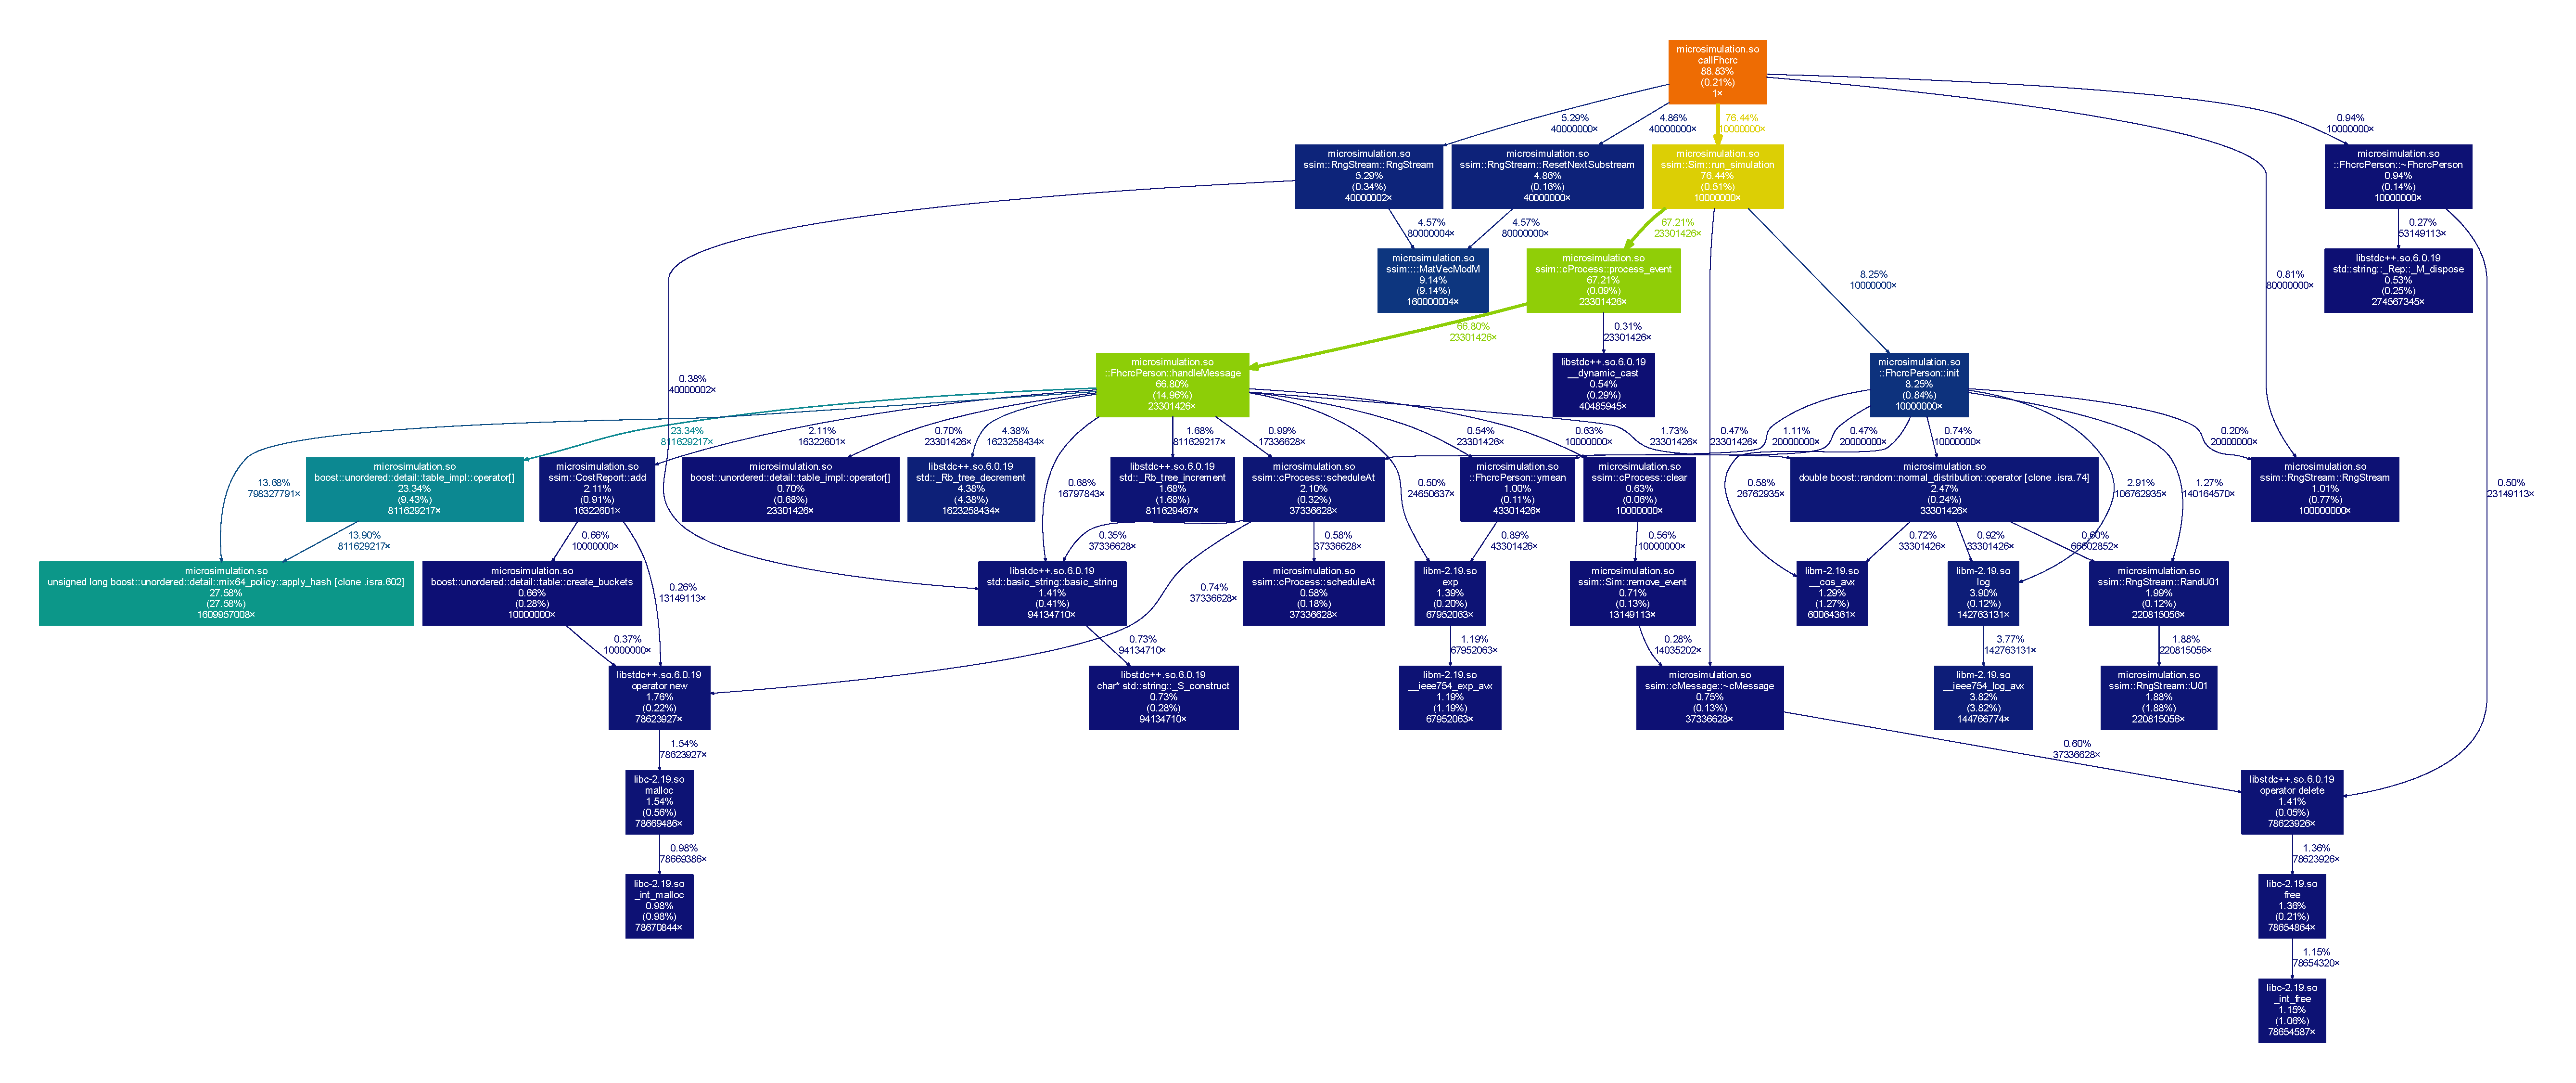
\includegraphics[height=0.50pp\textheight, angle=90]{images/profBaseLine.pdf}
  \caption{Valgrind measurements at baseline}
  \label{fig:simpleOpenMP}
\end{figure}


\subsection{Simple approach with OpenMP}

\begin{figure}[!htbp]
  \centering
  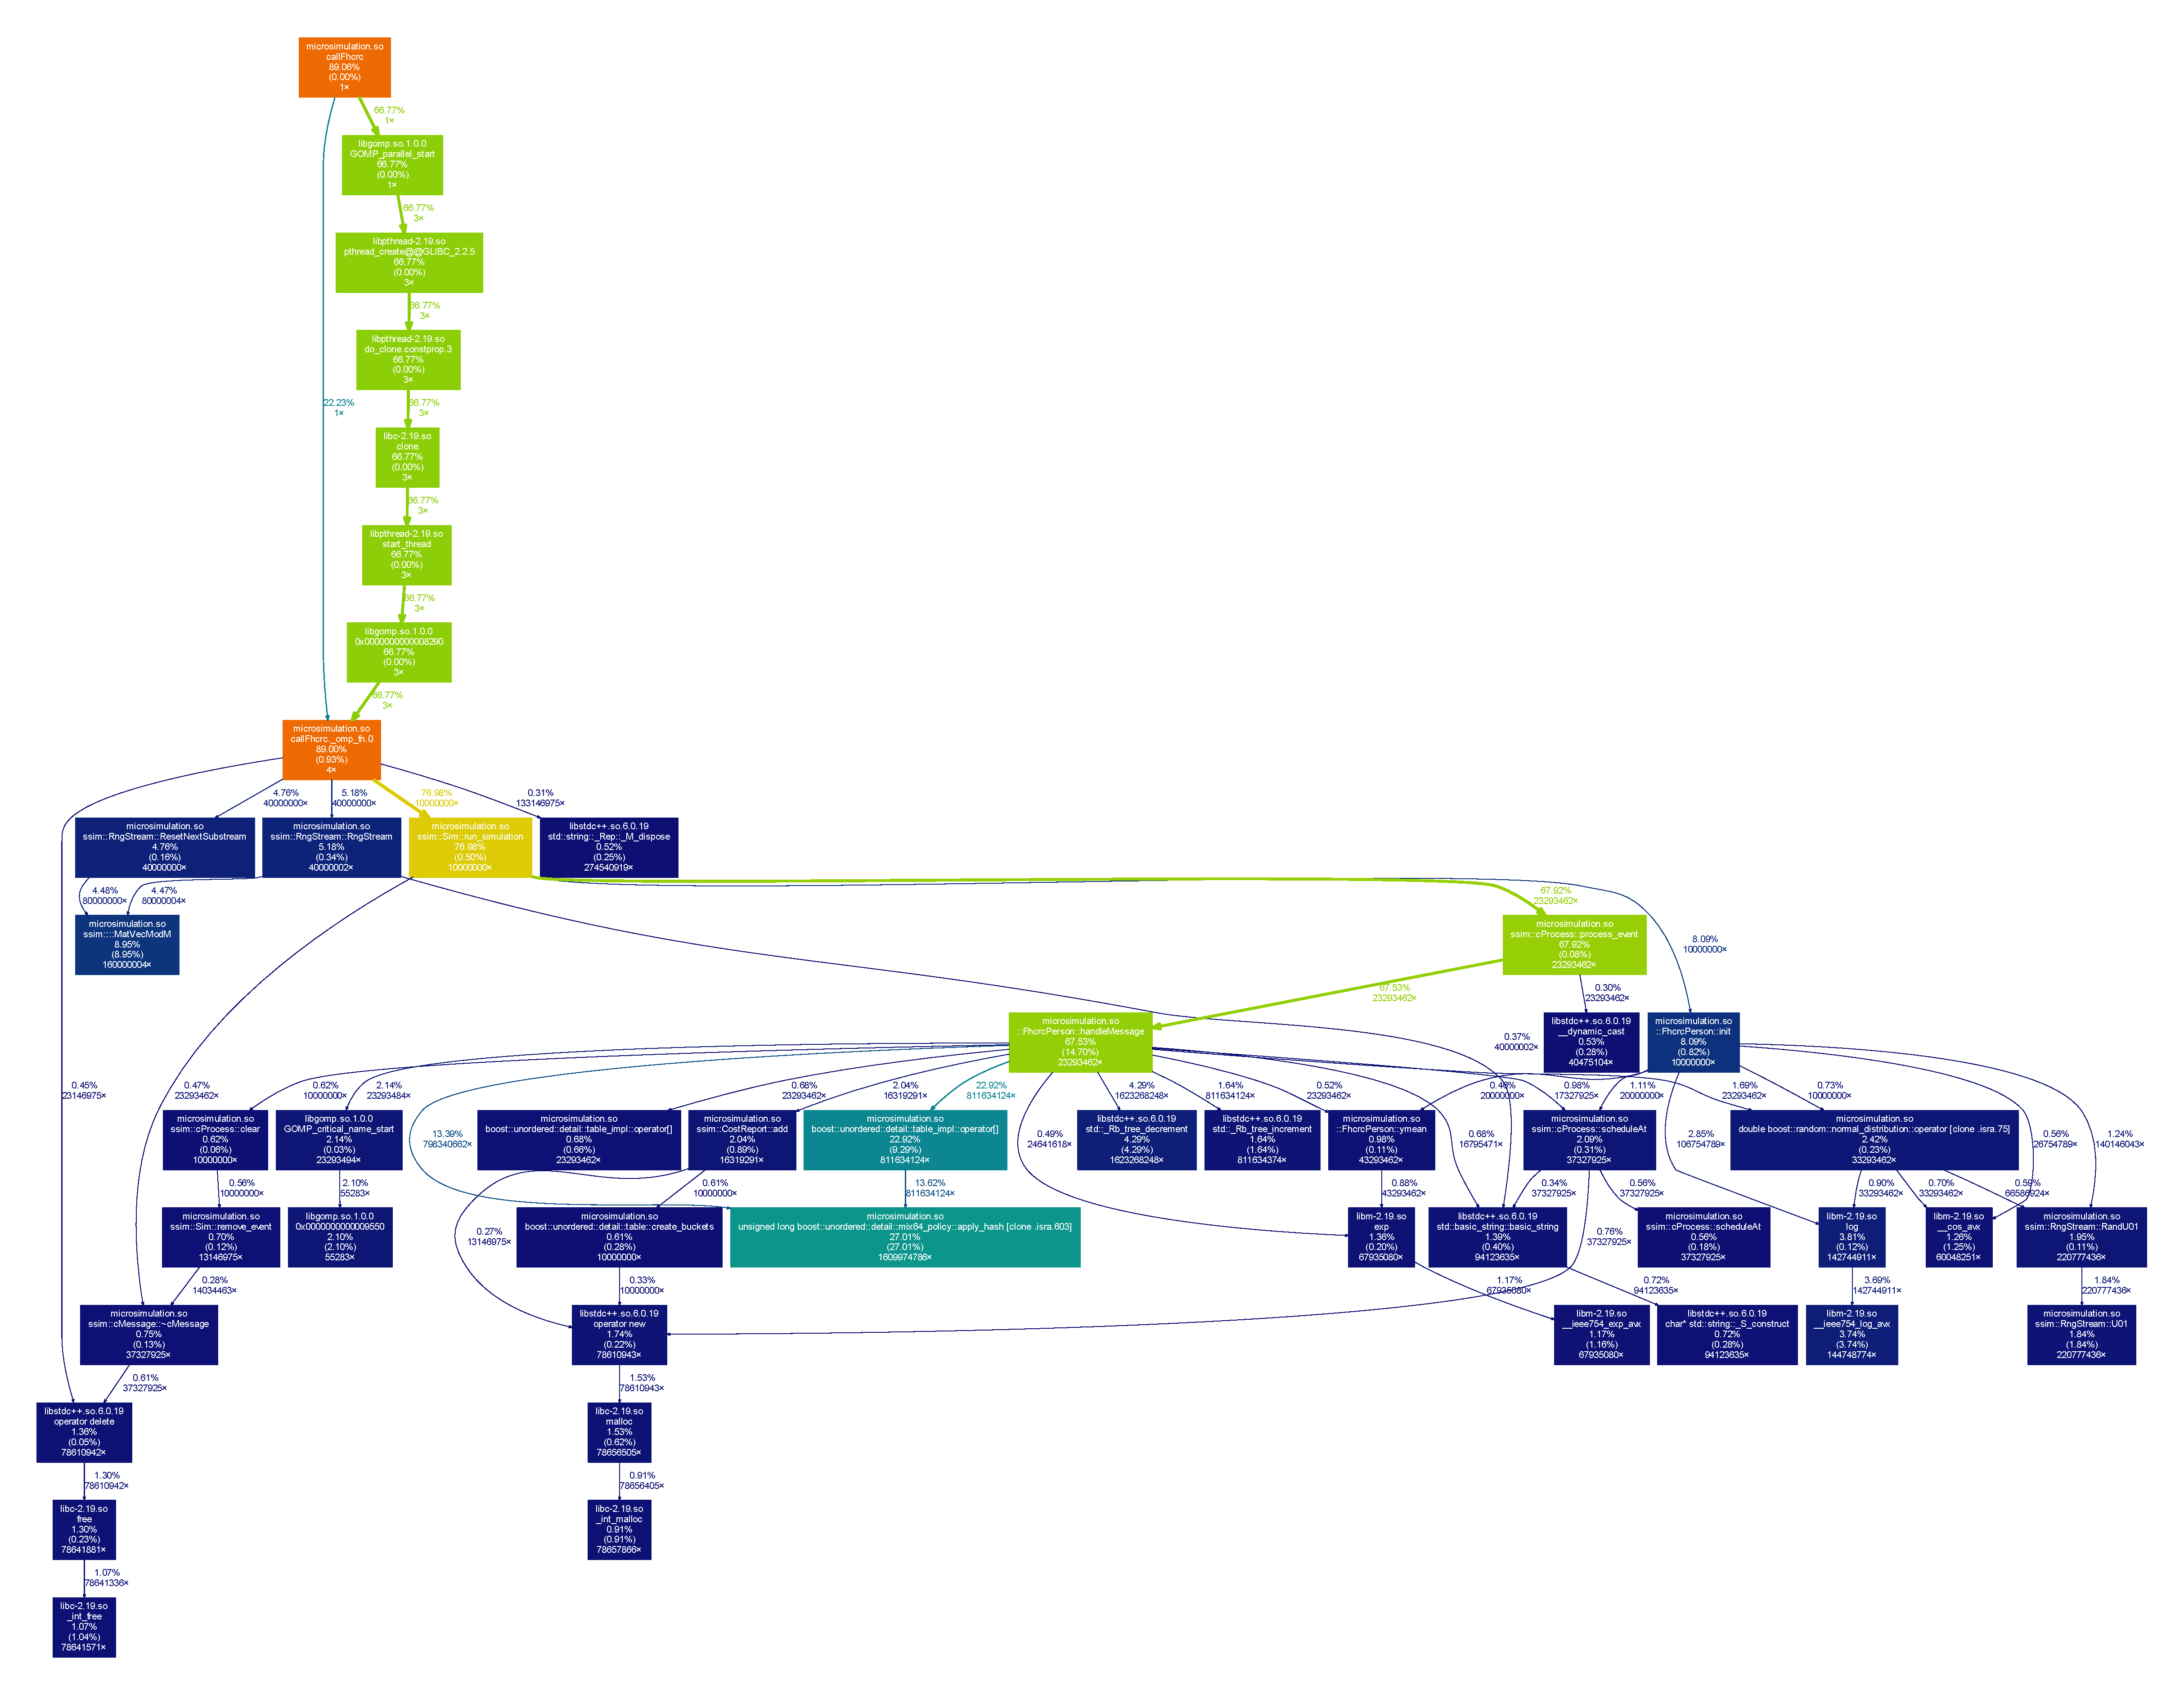
\includegraphics[height=0.85\textheight, angle=90]{images/profOpenMPSimple.pdf}
  \caption{Valgrind results of the simple openMP implementation}
  \label{fig:simpleOpenMP}
\end{figure}

Here the simulation loop is run in parallel whereas the data output
and some post-processing is run within a omp critical statement.

\subsection{Data output in parallel}


\subsection{Hybrid openMP and MPI}


%%% Local Variables:
%%% mode: latex
%%% TeX-master: "report"
%%% End:
